%!TEX root = ../thesis.tex
\chapter{Discussion}
\label{chapter_conclusion}

\section{Restatement of Contributions}
This dissertation has demonstrated video-based computational approaches that support tutorial creation and consumption from author demonstrations. Design and technical contributions of this work can be summarized as follows:

\begin{itemize}
  \item New instructional formats that consider learning factors. This dissertation contributed:
    \begin{itemize}
      \item Mixed-media tutorials composed of step-by-step static instructions and in-place video clips to demonstrate individual operations.
      \item Enhanced video playback that contains dynamic glyphs to provide viewers awareness to the upcoming input event.
    \end{itemize}
  \item Lightweight workflows in an easy-to-setup environment for amateur users to create effective instructions by demonstration.
    \begin{itemize}
      \item Methods for capturing, reviewing, and editing an instructional task with the support of software and capturing devices.
      \item User interfaces for annotating and editing a recorded demonstration.
      \item Multi-modal interfaces using motion, voice commands, and touch interaction to author step-by-step instructions while performing physical demonstrations.
    \end{itemize}
  \item Automatic or semi-automatic approaches using video and audio analysis that includes users in the loop to produce high-quality results.
    \begin{itemize}
      \item Algorithms of analyzing video, audio, and motion data using computer vision and signal processing approaches to segment a demonstration.
      \item Techniques for combining high-level user annotations with content analysis to generate concise instructions.
    \end{itemize}
\end{itemize}

% How to design tutorial systems appropriately for different situations
% * level of expertise of instructor, learner
% * what are you trying to make easier?

\section{Future Directions} %Remaining Challenges and


\subsection{Beyond Single-Author, Linear Authoring}
a team, beyond a single author for larger projects or tasks
Collaborative

branching

sharing - iterative

\subsection{Product Design Guidelines}
software learnability~\cite{Grossman:2009:SSL:1518701.1518803}
formal language
- now template, a set of techniques

\subsection{New Sensing Techniques}
Tango, Structure Sensor, Leap Motion

hand tracking~\cite{taylor-siggraph2016}
Fusion4D~\cite{dou-siggraph2016}

\subsection{Emerging Instructional Space}

Augmented and virtual reality systems are becoming available to end users via affordable forms. However, designing AR and VR experiences extremely requires expertise and efforts. As devices offer personalized effects supported by sensing and input techniques, we need new authoring tools that focus on delivering story-centric experiences. Tools should also enable both professionals and amateurs to create and iterate designs efficiently in an immersive 3D world. ...research what future AR and VR creation tools would look like with new authoring processes.

by demonstration
``Microsoft HoloLens with Autodesk MotionBuilder'' by Jasper Brekelmans, \url{https://www.youtube.com/watch?v=yfl7pwXftUs}, licensed under CC BY 2.0

\begin{figure*}[ht!]
  \centering
\begin{tabular}{cc}
  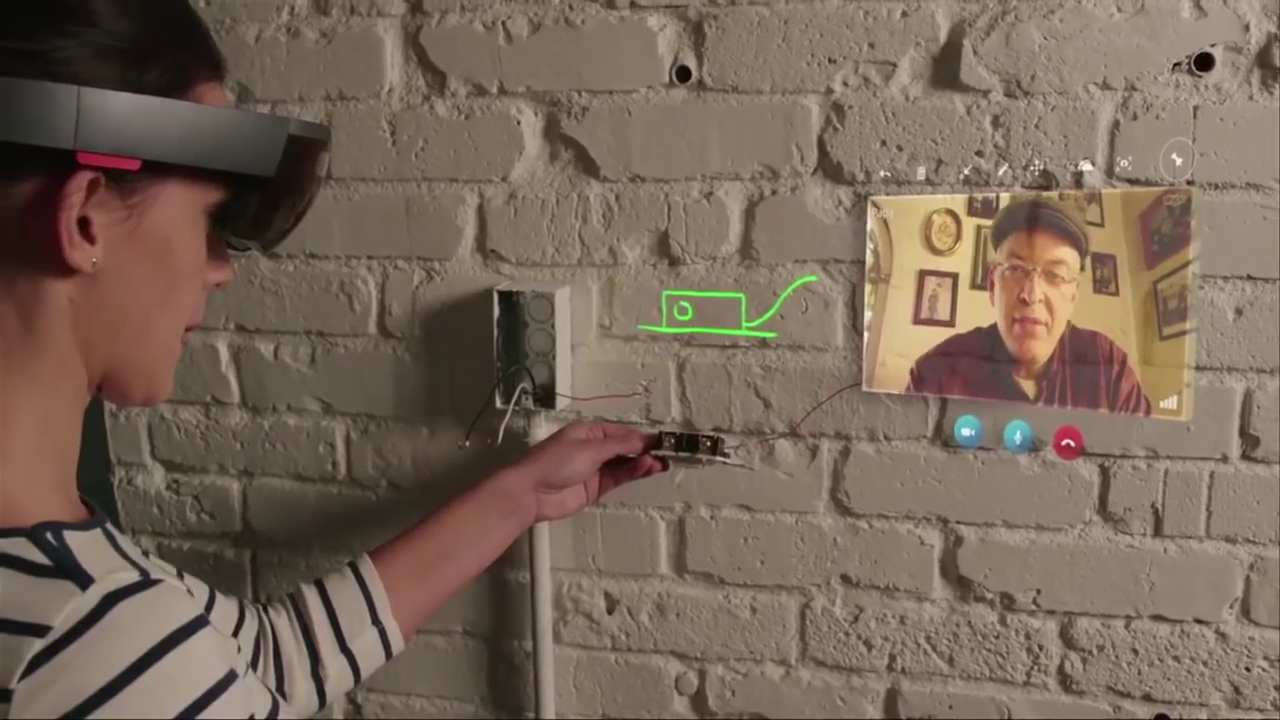
\includegraphics[width=0.4\textwidth]{\conclusion/fig/ar/hololens_fix1} &
  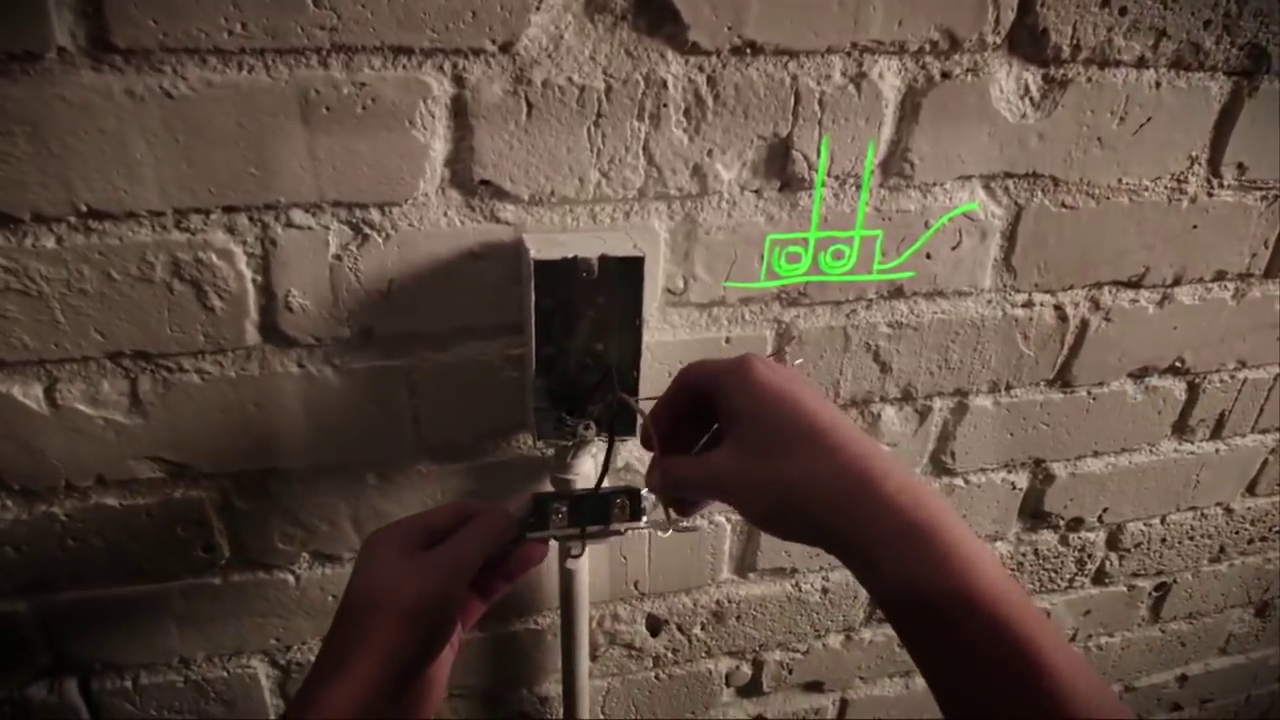
\includegraphics[width=0.4\textwidth]{\conclusion/fig/ar/hololens_fix2} \\
\multicolumn{2}{c}{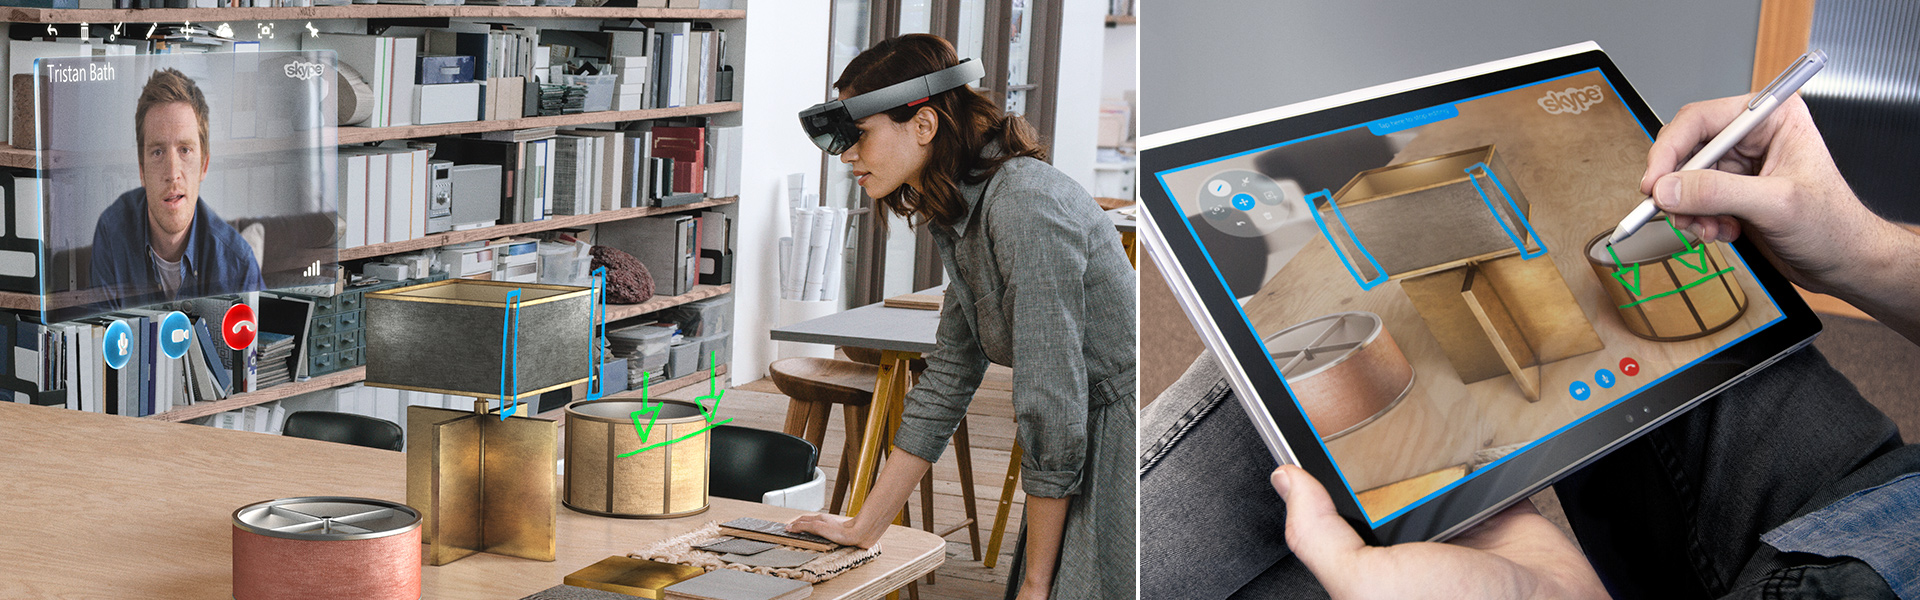
\includegraphics[width=0.82\textwidth]{\conclusion/fig/ar/hololens_skype} }
\end{tabular}
\caption{
  Microsoft's HoloLens~\cite{MicrosoftHoloLensSkype} has introduced an Augmented Reality application on providing real-time physical instructions from a remote instructor.
}
\end{figure*}

VR: capture physical instructions and share with others
authoring tools for immersive experiences

\section{Conclusion}
In this dissertation, we present video-based approaches designed for amateur users to produce and consume effective instructions from demonstrations. Using video and audio analysis techniques, our tools support recording, editing, and playback in a tutorial production process. We demonstrate results of our computer-generated tutorials from several domains, including software applications and physical activities. Our goal is to increase the quality of instructions created by tutorial authors and to support learners navigating and following the tutorials.
